\section{Zielsetzung}
In diesem Versuch sollen die Spaltbreiten eines Einfach- und Doppelspalts, anhand des Beugungsverhaltens von Licht, bestimmt werden.

\section{Theoretische Grundlagen}
Der Verlauf von Licht hinter einem Hindernis oder einem Schirm, mit Abmessungen im Größenbereich der Strahlungsdurchmesser, wird als Beugung bezeichnet. Das Licht kann dort Bereiche ausleuchten welche durch die geometrisch beschriebene Optik, scheinbar dunkel bleiben würden. Durch eine Wellenbetrachtung in Zusammenhang mit dem Huygensschen Prinzip lässt sich die Beugung an einem Spalt folgendermaßen erklären. 
\\
\newline
Auf den Spalt trifft eine Wellenfront wobei jeder Punkt dieser Welle nun nach dem Huygensschen Prinzip Ausgang einer neuen kugelförmigen Elementarwelle ist. Die Superposition dieser Elementarwellen bildet die neue Wellenfront und es kommt zu Interferenzerscheinungen welche gemessen werden können.
\\
\newline
Grundsätzlich gibt es zwei Versuchsanordnungen bei denen es zu Beugungen kommt, eine davon bietet sich mathematisch besonders an. Dies ist die Frauenhoferbeugung, bei ihr wird die Strahlungsquelle, sowie die Beobachtungsebene ins scheinbar Unendliche gelegt um eine möglichst parallele Strahlung zu erhalten. Dies kann gut durch einen großen Abstand zwischen Beobachtungsebene und Spalt, sowie einer geeigneten Strahlungsquelle, also beispielsweise einem Laser, erzeugt werden. Der Vorteil liegt darin, dass bei der Frauenhoferbeugung die Interferenz an einem Punkt $P$ in der Beobachtungsebene nur von Licht mit festem Beugungswinkel abhängt. Bei der sogenannten Fresnelbeugung ist diese Vereinfachung nicht möglich. Eine schematische Abbildung des Strahlengangs bei Frauenhoferbeugung ist in Abbildung \ref{fig:fig1} dargestellt.
\begin{figure}
    \centering
    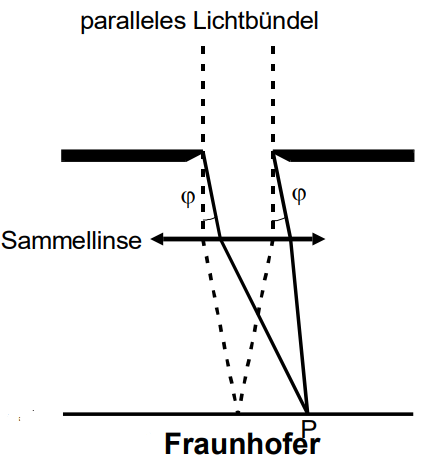
\includegraphics[width=0.4\textwidth]{bilder/1.png}
    \caption{Schematische Abbildung der Frauenhoferbeugung am Einfachspalt. \cite{skript}} 
    \label{fig:fig1}
\end{figure}
Die gemessenen Werte der Intensität bei unterschiedlichen Winkeln lassen sich mit einer theoretischen Intensitätsfunktion $I(\phi)$ überprüfen. Diese Funktion wird im Folgenden erläutert.

\subsection{Berechnung der Intensität am Einzelspalt}
Im Folgenden wird nur noch der Fall für die Frauenhoferbeugung behandelt. 
Eine von einem Laser erzeugte ebene Welle falle nun aus der z-Richtung ein und oszilliert in x-Richtung. Die Feldstärke $A(z,t)$ ist Lösung der Wellengleichung und lässt sich folgendermaßen schreiben.
\begin{equation}
    \label{eqn:eq1}
   A(z,t)  = A_{0} \text{exp}\left(i\left(\omega t - \frac{2\pi z}{\lambda} \right)\right)
\end{equation}
 Die Annahme der Frauenhoferbeugung benötigt die Bedingung, dass der Schirmabstand $d >> b$ ist, wobei $b$ die Spaltbreite angibt. Für die Amplitude bei einem bestimmten Beugungswinkel $\phi$ müssen nun alle Strahlbündel mit diesem Winkel aufsummiert werden, dabei muss beachtet werden, dass zwei verschiedene Strahlbündel auch einen Phasenunterschied, aufgrund ihres Gangunterschiedes $s$ haben. Die Phasendifferenz lässt sich folgendermaßen angeben.
 \begin{equation}
     \delta = \frac{2\pi s}{\lambda} = \frac{2\pi x \cdot \text{sin}(\phi) }{\lambda}
 \end{equation}
Dabei wurde der Gangunterschied $s$ durch geometrische Überlegungen in Abbildung \ref{fig:fig2} für zwei Punkte im Spalt mit Abstand $x$ eingesetzt, da im Folgenden über alle x-Werte im Spalt integriert wird.
Nun kann die Phasendifferenz in die Gleichung \eqref{eqn:eq1} eingesetzt und integriert werden.
\begin{equation}
B(z, t, \phi) =  A_{0} \int_{0}^{b} \text{exp} \left( i(\left( \omega t - \frac{2\pi z}{\lambda} + \delta\right)\right)
\end{equation}
Die Lösung lautet.
\begin{equation}
    \label{eqn:eq2}
    B(z, t, \phi) =  A_{0} \text{exp}\left(i\left(\omega t - \frac{2\pi z}{\lambda} \right)\right) \cdot \text{exp}\left( \frac{i \pi b \cdot \text{sin}(\phi)}{\lambda}\right) \cdot \frac{\lambda}{\pi \cdot \text{sin}(\phi)} \cdot \text{sin}\left( \frac{\pi b  \cdot \text{sin}(\phi)}{\lambda} \right)
\end{equation}
Diese Gleichung beschreibt nun also den Schwingungszustand eines beliebigen Punktes hinter dem Spalt. Von Vorteil ist dabei, dass die beiden Exponentialterme nur Phasenfunktionen sind und sie
beim quadrieren für die Bestimmung der Intensität keine Auswirkung haben. Die Amplitude lässt sich in diesem Fall nur schwer messen, allerdings kann mit der zeitlich gemittelten Intensität $I(\phi)$ gearbeitet werden, diese ist proportional zu dem Betragsquadrat von der 
Funktion $  B(z, t, \phi)$.
\begin{equation}
    \label{eqn:eq3}
I(\phi) \propto B^{2}(\phi) = A_{0}^{2} b^{2} \left( \frac{\lambda}{\pi b \cdot \text{sin}(\phi)}\right)^{2} \cdot \text{sin}^{2}\left(\frac{\pi b \cdot \text{sin}(\phi)}{\lambda}\right)
\end{equation}
Durch das Quadrieren ändern sich ebenfalls die Orte der Nullstellen vom Sinusanteil aus Gleichung \eqref{eqn:eq2} nicht. Der Term beschreibt einen Sinus cardinalis und hat die Nullstellen bei.
\begin{equation*}
\text{sin}(\phi_{n}) = \frac{n \lambda}{b} \quad \quad \bigl| n \in \mathbb{Z}
\end{equation*}
\begin{figure}
    \centering
    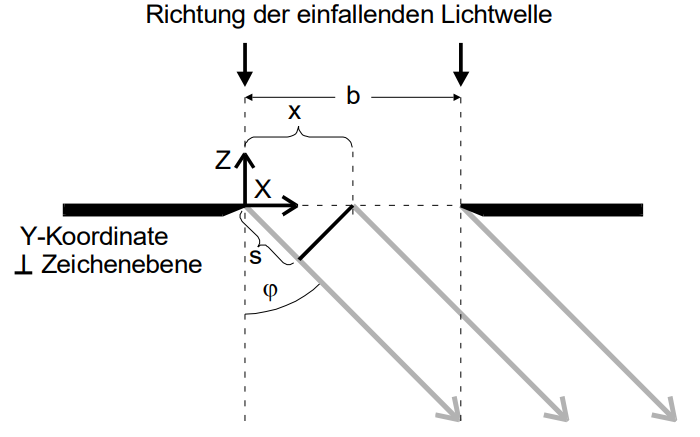
\includegraphics[width=0.5\textwidth]{bilder/2.png}
    \caption{Geometrische Betrachtung des Einfachspalts. \cite{skript}} 
    \label{fig:fig2}
\end{figure}
\subsection{Berechnung der Intensität am Doppelspalt}
Analog kann eine Intensitätsfunktion für den Doppelspalt bestimmt werden, dabei wird durch Überlagerung von zwei Einfachspalten ein ähnlicher Ausdruck gewonnen.
Wichtig ist, dass weiterhin die Bedingungen für die Frauenhoferbeugung gelten müssen. Der Spaltabstand zwischen den beiden Einfachspalten ist im Folgenden als $s$ bezeichnet.
Die Intensität ergibt sich zu.
\begin{equation}
    \label{eqn:eq4}
    I(\phi) \propto B^{2}(\phi) = 4 \cdot \text{cos}^{2}\left( \frac{\pi s \cdot \text{sin}(\phi)}{\lambda}\right) \cdot \left( \frac{\lambda}{\pi b \cdot \text{sin}(\phi)}\right)^{2} \cdot \text{sin}^{2}\left( \frac{\pi b \cdot \text{sin}(\phi)}{\lambda}\right)
\end{equation}
Erkennbar ist, dass die vorherige Intensitätsverteilung des Einfachspalts in dem Term enthalten ist mit einem zusätzlichen Term $\text{cos}^{2}$. Die Intensität eines Doppelspalts wird also durch die Intensität
der Einzelspalte moduliert.
Es kommen allerdings weitere Nullstellen durch den Kosinusterm hinzu. Diese liegen bei.
\begin{equation}
\phi(k)= \text{arcsin}\left(\frac{2k + 1}{2s}\right)\cdot \lambda \quad \quad \bigl| k \in \mathbb{N}
\end{equation}

\subsection{Zusammenhang zur Fouriertransformation}
Mathematisch kann die Berechnung der Amplitudenverteilung auch anders bestimmt werden. Es gibt einen Zusammenhang zwischen der Funktion $B(\phi)$ und der sogenannten Aperturfunktion. Die Aperturfunktion ist hier eine konstante Funktion 
für $ 0 \leq x \leq b$, welche die Beugungsebene der einfallenden Welle beschreibt.
Die Fouriertransformierte einer konstanten Funktion über ein kompaktes Intervall ist im Allgemeinen der Sinus cardinalis und damit lässt sich ein Zusammenhang über die Fouriertransformation erwarten.
Eine allgemeine Fouriertransformation sieht folgendermaßen aus.
\begin{equation}
\hat{f}(\zeta) = \int_{-\infty}^{\infty} f(x) \text{exp}(-ix\zeta) \text{d}x
\end{equation}
Mit der Anwedungen auf die Aperturfunktion ergibt sich.
\begin{equation}
    \hat{f}(\zeta) = \frac{2A_{0}}{\zeta} \text{exp}\left(\frac{i \zeta b}{2}\right) \text{sin}\left(\frac{\zeta b}{2}\right)
\end{equation}
Dieses Ergebniss stimmt mit dem nur von $\phi$ abhängigen Teil von $B(z, t, \phi)$ aus Gleichung \eqref{eqn:eq2} überein, wenn $\zeta$ als
\begin{equation}
\zeta = \frac{2\pi \text{sin}(\phi)}{\lambda}
\end{equation}
identifiert wird. Anhand einer Fouriertransformation lässt sich also durch die Eigenschaft der Öffnungsweite direkt eine Beschreibung für die Schwingung an allen Orten finden. Solange die betrachte Funktion absolut integrierbar ist existiert die Fouriertransformation und umgekehrt
kann auch aus der Amplitudenfunktion die Aperturfunktion berechnet werden. 